% Don't touch this %%%%%%%%%%%%%%%%%%%%%%%%%%%%%%%%%%%%%%%%%%%
\documentclass[11pt]{article}
\usepackage{fullpage}
\usepackage[left=0.9in,top=0.9in,right=0.9in,bottom=0.9in,headheight=3ex,headsep=3ex]{geometry}
\usepackage{graphicx}
\usepackage{float}
\usepackage{adjustbox}
\usepackage{tikz}
\usetikzlibrary{positioning}
\usetikzlibrary{snakes}
\usetikzlibrary{calc}
\usetikzlibrary{arrows}
\usetikzlibrary{decorations.markings}
\usetikzlibrary{shapes.misc}
\usetikzlibrary{matrix,shapes,arrows,fit,tikzmark}


\newcommand{\blankline}{\quad\pagebreak[2]}
%%%%%%%%%%%%%%%%%%%%%%%%%%%%%%%%%%%%%%%%%%%%%%%%%%%%%%%%%%%%%%

% Modify Course title, instructor name, semester here %%%%%%%%

\title{ECN 453: Homework 3 - solutions}
%\author{\textbf{Due: Start of class Monday 29th November.} \\
%\textbf{You can work in groups of up to 3 people (hand in one solution per group).} }
%\date{Fall, 2021}

%%%%%%%%%%%%%%%%%%%%%%%%%%%%%%%%%%%%%%%%%%%%%%%%%%%%%%%%%%%%%%

% Don't touch this %%%%%%%%%%%%%%%%%%%%%%%%%%%%%%%%%%%%%%%%%%%
%\usepackage[sc]{mathpazo}
\linespread{1.3} % Palatino needs more leading (space between lines)
\usepackage[T1]{fontenc}
\usepackage[mmddyyyy]{datetime}% http://ctan.org/pkg/datetime
\usepackage{advdate}% http://ctan.org/pkg/advdate
%\newdateformat{syldate}{\twodigit{\THEMONTH}/\twodigit{\THEDAY}}
\newsavebox{\MONDAY}\savebox{\MONDAY}{Mon}% Mon
\newcommand{\week}[1]{%
%  \cleardate{mydate}% Clear date
% \newdate{mydate}{\the\day}{\the\month}{\the\year}% Store date
  \paragraph*{\kern-2ex\quad #1, \syldate{\today} - \AdvanceDate[4]\syldate{\today}:}% Set heading  \quad #1
%  \setbox1=\hbox{\shortdayofweekname{\getdateday{mydate}}{\getdatemonth{mydate}}{\getdateyear{mydate}}}%
  \ifdim\wd1=\wd\MONDAY
    \AdvanceDate[7]
  \else
    \AdvanceDate[7]
  \fi%
}
\usepackage{setspace}
\usepackage{multicol}
%\usepackage{indentfirst}
\usepackage{fancyhdr,lastpage}
\usepackage{url}
\pagestyle{fancy}
\usepackage{hyperref}
\usepackage{lastpage}
\usepackage{amsmath}
\usepackage{layout}
\renewcommand{\theenumi}{\alph{enumi}}


\lhead{}
\chead{}
%%%%%%%%%%%%%%%%%%%%%%%%%%%%%%%%%%%%%%%%%%%%%%%%%%%%%%%%%%%%%%

% Modify header here %%%%%%%%%%%%%%%%%%%%%%%%%%%%%%%%%%%%%%%%%
\rhead{\footnotesize ECN 453: Homework 3}

%%%%%%%%%%%%%%%%%%%%%%%%%%%%%%%%%%%%%%%%%%%%%%%%%%%%%%%%%%%%%%
% Don't touch this %%%%%%%%%%%%%%%%%%%%%%%%%%%%%%%%%%%%%%%%%%%
\lfoot{}
\cfoot{\small \thepage/\pageref*{LastPage}}
\rfoot{}

\usepackage{array, xcolor}
\usepackage{color,hyperref}
\definecolor{clemsonorange}{HTML}{EA6A20}
\hypersetup{colorlinks,breaklinks,linkcolor=clemsonorange,urlcolor=clemsonorange,anchorcolor=clemsonorange,citecolor=black}

\date{} 

\begin{document}
\maketitle

%\paragraph{Instructions} Please neatly write your answers, staple them together, and submit this homework at the start of class on Monday 29th November.\footnote{If you can't come to class you can email me your solutions.} If the work is too messy/hard to read it will not be graded. I encourage you to talk to your classmates about the homework, but make sure you can do all the problems. Don't forget to put the names of everyone in your group on the front. If you have questions come and talk to me in office hours, after class, or by email: nvreugde@asu.edu. Good luck!

\subsection*{1. New technology and market structure (30 points)}
Consider an industry with market demand $Q=a-p$ and an infinite number of potential entrants with access to the same technology. Initially, the technology is given by $C=F+cq$. A new technology allows for a lower marginal cost $c'<c$ at the expense of a higher fixed cost $F'>F$.
\\

Given $a=10, F=2, F'=3,c=2,c'=1$.

\begin{enumerate}

\item 

Use the following formula (from the lecture slides) for the number of firms $n$:

\begin{align*}
	n = \left[ (a-c) \sqrt{\frac{S}{F}} - 1 \right]
\end{align*}
Then, use the following formula (from the lecture slides) for the price, given the above number of firms:
\begin{align*}
	p = \frac{a+nc}{n+1}
\end{align*}


\underline{Under the old technology}:

Here, $a=10,c=2,S=1,F=2$. So: $n=\left[ (10-2)\sqrt{1/2}-1 \right] = 4$.

Then, equilibrium price under old technology:
\begin{equation*}
	p = \frac{10+4 \times 2}{4+1}=3.6
\end{equation*}

\underline{Under the new technology}:

Here, $a=10,c=1,S=1,F=3$. So: $n=\left[ (10-1)\sqrt{1/3}-1 \right] = 4$.

Then, equilibrium price under new technology:
\begin{equation*}
p = \frac{10+4 \times 1}{4+1} = 2.8
\end{equation*}

\end{enumerate}

\newpage

\subsection*{2. Repeated games (50 points)}
Consider the following game and suppose that it is repeated an infinite number of times. Players have a discount value of $\delta$. 
\begin{figure}[h]
	\centering
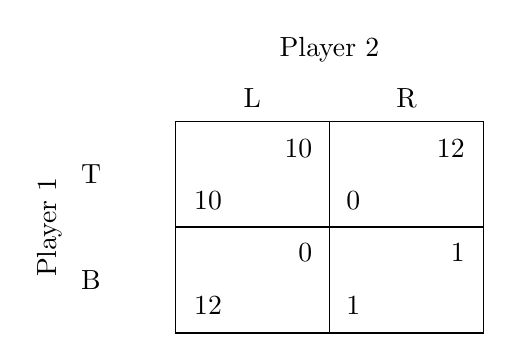
\begin{tikzpicture}
	\matrix[matrix of math nodes,
	every odd row/.style={align=right},every evenrow/.style={align=left},every node/.style={text width=1.5cm},row sep=0.2cm,column sep=0.2cm,ampersand replacement=\&] (m) {
		10\&12 \\
		10\&0 \\
		0 \&1 \\
		12 \&1\\
	};
	\draw (m.north east) rectangle (m.south west);
	\draw (m.north) -- (m.south);
	\draw (m.east) -- (m.west);
	
	% Player 1
	\coordinate (c) at ($(m.north west)!0.25!(m.south west)$);
	\coordinate (d) at ($(m.north west)!0.75!(m.south west)$);
	\node[left=2pt of c,text width=1cm]  {T};
	\node[left=2pt of d,text width=1cm]  {B};
	
	% Player 2
	\coordinate (a) at ($(m.north west)!0.25!(m.north east)$);
	\coordinate (b) at ($(m.north west)!0.75!(m.north east)$);
	\node[above=5pt of a,anchor=base] {L};
	\node[above=5pt of b,anchor=base] {R};
	
	\node[above=18pt of m.north] (firm b) {Player 2};
	\node[left=1.6cm of m.west,rotate=90,align=center,anchor=center] {Player 1};
	
	%\node[above=5pt of firm b]  {Payoff Matrix};
\end{tikzpicture}
\end{figure}

\begin{enumerate}

\item 

Equilibrium payoff:
\begin{equation*}
	\Pi = 10 + \delta10 + \delta^2 10 + \delta^3 10 +.... = \frac{10}{1-\delta}
\end{equation*}

Deviation payoff:
\begin{equation*}
\Pi' = 12 + \delta + \delta^2 + \delta^3  +.... = 12 + \frac{\delta}{1-\delta}
\end{equation*}

Therefore, for collusion to sustain, we need:
\begin{align*}
	\Pi \geq \Pi' \\
	\frac{10}{1-\delta} \geq 12 +  \frac{\delta}{1-\delta} \\ 
	10 - \delta \geq 12(1-\delta) \\
	\delta \geq \frac{2}{11}
	\end{align*}


\item 
Equilibrium payoff is the same.

Deviation payoff:

\begin{equation*}
\Pi' = 12 + 0\delta + 0\delta^2 + 0\delta^3  +.... = 12 
\end{equation*}

Therefore, for collusion to sustain, we need:
\begin{align*}
\Pi \geq \Pi' \\
\frac{10}{1-\delta} \geq 12 \\ 
10 \geq 12(1-\delta) \\
\delta \geq \frac{2}{12}
\end{align*}

\item The players sustain collusion on (T,L) using the grim trigger punishment of playing (B,R) in all future periods, and the discount factor $\delta$ indexes how much agents care about this future punishment. Since in Part b, the punishment is harsher than in Part a, (since the players get (0,0) for all future periods rather than (1,1)), collusion can be sustained for lower discount factors.

\end{enumerate}

\end{document}